\chapter{Structured priors for brain decoding and functional segmentation: the models}\label{chap:structured_priors}
\markright{{~{\rm \ref{chap:structured_priors}}. Structured priors for analyzing brain data}\hfill}{}

\minitoc

\section{Introduction to brain decoding}
As already discussed in chapter \ref{chap:bigpic}, functional brain imaging provides a distinctive opportunity to study brain functional architecture, while being minimally invasive, and is thus well-suited for the challenging study of the spatial layout of neural coding. Different modalities exist, each one having specific spatial and temporal resolutions; among them Functional Magnetic Resonance Imaging (fMRI)~\citep{agawa1990,ogawa1990b} has emerged as a fundamental modality for brain imaging, striking a good balance between spatial and temporal resolution.  fMRI images are pre-processed, and modeled through a general linear model (GLM), that takes into account the different experimental conditions and the dynamics of the haemodynamic response in the design matrix. The resulting model parameters, a.k.a. activation maps, represent the influence of the different experimental conditions on local fMRI signals.

\paragraph{The standard approach.}
The standard approach used for analyzing these activation maps is called classical inference, and relies on a mass-univariate statistical tests (one for each voxel), yielding the so-called statistical parametric maps (SPMs)~\citep{friston1994statistical}. Such maps are of particular interest in cognitive neuroscience, as they open the door to localizing the voxels that are significantly active for any combination of experimental conditions, and thus are probably implied in the underlying neural code of the cognitive processes. However, this classical inference suffers from multiple comparisons issues. Also, it does not take into account the multivariate structure of the fMRI data.

\begin{pagefigure}
  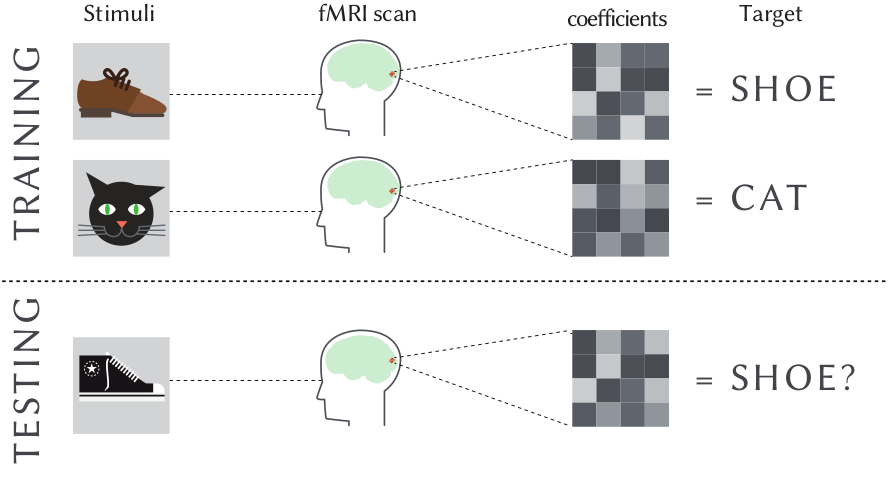
\includegraphics[width=1\linewidth]{figures/decoding.png}
  \caption{\textbf{Decoding} models mine
patterns of activity to discriminate
between cognitive states~\citep{dehaene1998}. Different
activation patterns reflect different mental states. For example,
those associated with different images viewed by the subject.
In a training phase, the classifier will
learn to discriminate between brain activity measured under different
cognitive states. In the testing phase the generalization performance of the trained model is
quantified by evaluating the classifier on the testing set and comparing
the output of the classifier with the true labels associated with
the stimuli. % One can map the accuracy of the decoder to ....
Adapted from ~\citep{pedregosa2015feature}}.
\end{pagefigure}

\paragraph{Inference inference (or ``brain reading'').}
An alternative approach called \textit{inverse inference} (or ``brain-reading'')~\citep{dehaene1998,cox2003}, has been proposed in order to cope with the limitations of the afore-mentioned classical inference. Inverse inference relies on a pattern recognition, and aims at decoding the neural code by using machine-learning methods. Based on a set of brain activation maps, inverse inference builds a predictive model that can be used for predicting a behavioral target (age, sex, IQ, etc.) for a new set of images. The prediction accuracy of the model is used as a measure of the quantity of information about the cognitive task shared by the voxels. By construction, this approach is multivariate, and can provide more sensitive analysis than standard statistical parametric mapping procedure [Kamitani 05, Haynes 06]. Several methods have been tested for classification or regression of activation images (Linear Discriminant Analysis -- LDA, Support Vector Machines -- SVM, Lasso, Elastic net regression, and many others), but, in this problem, the major bottleneck remains the localization of predictive regions within the brain volume. Additionally, we have to deal with the curse of dimensionality, as the number of features (voxels, regions) is much larger ($\sim 10^5-10^6$ ) than the numbers of sample (images) ($\sim 10^2 - 10^3$ ), the latter being limited by the cost of acquisition. Thus the prediction method may overfit the training set and thus not generalize well to new samples.

\section{Sparsity and structure-inducing priors: towards intepretable multi-variate models}
To cope with the high dimensionality of the data, the learning method has to be
regularized. However, the spatial structure of the image is not
taken into account in standard regularization methods, so that the
extracted features are often hard to interpret.
Sparsity and spatial smoothness inducing priors can used to
perform jointly the prediction of a target variable and region
segmentation in multivariate analysis settings. Sparsity can be enforced by
penalizing the (sum of) absolute values of the regression coefficients, leading to the
so-called Lasso model. Smoothness can achieved in penalizing the spatial gradient of
the regression coefficients, to enforce smooth regions (``blobs'').
The Total-variation (TV)~\citep{rudin1992nonlinear} penalty has
proven to be particularly powerful for realizing such effects. Laplacian regularization
is an easier means to this end (because in leads to a differentiable problem),
but have sub-optimal rates for noisy signal recovery~\citep{minimaxtv}, and the visual effect is less appealing.

In the context of neuro-imaging, sparsity and smoothness have been compiled to yield
regression coefficients which are faithful to known neurobiological organization of the brain,
while alleviating the risk of over-fitting due to inherently small-sample settings.
Specifically, it has been shown that one can employ priors like TV-$\ell_1$
~\citep{baldassarre2012,gramfort2013}, TV-ElasticNet~\citep{dubois2014predictive},
and GraphNet ~\citep{grosenick2013}
(aka Smooth-Lasso~\citep{hebiri2011})
%\footnote{Henceforth, we will use GraphNet and S-Lasso
%interchangeably.}
to regularize regression and classification
problems in brain imaging. TV has also been employed to enhance the estimation of the voxel-wise \textit{Hurst exponent}~\footnote{$H := \lim_{N \rightarrow \infty}\frac{\mathbb E(r_N/\sigma_N)}{\log N}$,
where $r_N$ is the empirical range (i.e max value minus min value) of the first $N$ values in a time-series, and $\sigma_N$ is their standard deviation. For example in 1D, white noise has $H = -1/2$.},
as a measure of temporal self-similarity in brain dynamics~\citep{pelle2016multivariate}.

\paragraph{Notation.} We denote by ${\y} \in \mathbb{R}^{n}$ the targets to
be predicted (age, sex, IQ, etc.); the \textit{design matrix}
${\X}\in\mathbb{R}^{n \times p}$ are the masked (see Fig. \ref{fig:masking})
brain images related to the presentation of different
stimuli, or other brain acquisition (e.g gray-matter concentration
maps from anatomy, etc.). The integer $p$ is the number of voxels,
and $n$ the number of samples (images). In brain imaging, $n \ll p$;
typically, $p \sim 10^3-10^6$ (in full-brain analysis),
while $n \sim 10-10^3$ ($n$ being limited by the cost of acquisition,
etc.). $\nabla_x$ will denote the discrete spatial gradient operator
along the $x$-axis, $\nabla_y$ along the $y$-axis, etc.
Thus, at a voxel $j$, the spatial gradient of an image $\B{w}$ is a vector ${\nabla} {\w}(j) := [\nabla_{x} {\w}(j), \nabla_{y} {\w}(j), \nabla_{z} {\w}(j)]$, $\forall \w \in \mathbb R^p$.
This defines a linear operator $\nabla \in \mathbb R^{3p \times p}$ (the discrete 3D spatial gradient operator) from $\mathbb R^p$ to $\mathbb R^{3p}$. For a mixing constant $\rho \in [0, 1]$, $\nabla_\rho \in \mathbb R^{4p \times p}$ will denote the identity-augmented version of $\nabla$, defined by ${\nabla_\rho} {\w} := [(1-\rho)\nabla \w, \rho \w] \in \mathbb R^{4p}$.

%% Let $\mathcal P \subset \mathbb{R}^3$ be
%% the 3D image domain representing the region occupied by the brain --or
%% ROI (region of interest) thereof-- under  study, discretized regularly
%% on a finite grid.

  \begin{figure}[!htb] 
  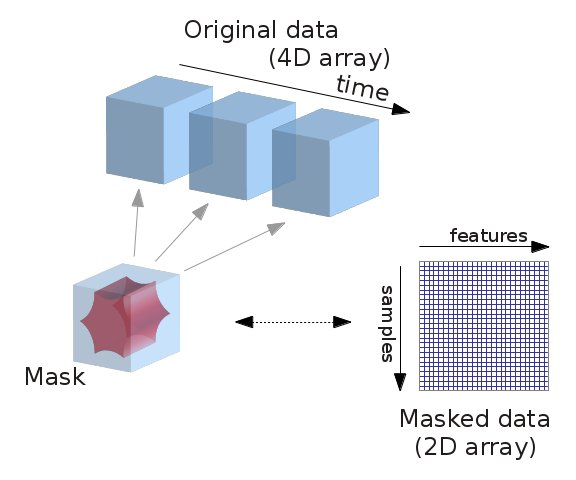
\includegraphics[width=1\linewidth]{figures/masking.jpg}
  \caption{\textbf{Masking} of volumic brain data (4D = 3D space + 1 \textbf{time} or \textbf{samples})
    to produce a design matrix required in standard machine learning (clustering, classification, regression, etc.). Each 3D volume considered is a sample point. The values of the voxels in this volume that lie in the mask are collected into a \textbf{feature vector}. All these vectors are vertically stacked to produce an $n$-by-$p$ design matrix $\X$, where $p$ is the number of voxels in the mask. The mask can be just the region of the 3D cube occupied by the brain, or a subset of such. In the latter case, this typically corresponds to Region-of-Interests (ROIs) deemed to be interesting for an experiment. The former case is referred to as ``full brain'', and the mask typically contains up to $p = $ millions of voxels. See ~\citep{abraham2014machine} for more details.}
  \label{fig:masking}
\end{figure}

\section{SpaceNet: sparse structured models for brain data}
Over time, a number of spatially regularized linear models have been proposed. These are mainly: Total-Variation (TV)~\citep{michel2011tv}, TV-$\ell_1$~\citep{baldassarre2012,gramfort2013}, GraphNet  ~\citep{grosenick2013,hebiri2011},
TV-ElasticNet~\citep{dubois2014predictive}, Sparse Variation~\citep{eickenberg2015total}, and social-sparsity~\citep{kowalski2013social,varoquaux2016social}. These can all be synthesized into a general framework, referred to as \textit{SpaceNet}~\citep{spacenetohbm}, as follows

\begin{figure}[!htbp]
  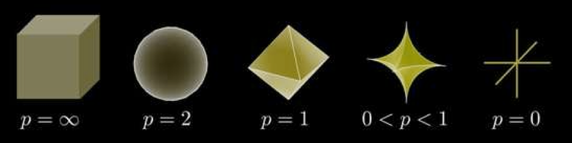
\includegraphics[width=1\linewidth]{figures/balls.png}
  \caption{$\ell_p$ unit ball for various values of $p$. The kinks
    in the cases $0 \le p \le 1$ impose sparsity. One notes however that, the
  cases $0 \le p < 1$ lead to non-convex intractable optimization problems.}
\end{figure}

\begin{equation}
  \underset{\w \in \mathbb R^p}{\text{minimize }}E(\w) := \ell(\y,\X\w) + \alpha \mathcal P(\w).
    \label{eq:opt_pb}
\end{equation}
The coefficients ${\w}$ define a spatial map in over the brain (one value per voxel).
The term {$\ell(\y,\X\w)$} is the
  {loss / data-fit term}. Popular choices include:
  $$
  \ell(\y,\X\w) = \frac{1}{n}\sum_{i=1}^n\begin{cases}\frac{1}{2}(\B{X}^T_i\w - y_i)^2,
    &\mbox{ \text{ for least-squares regression}}\\
    \log(1+\exp(-y_i\X_i^T\w)),
    &\mbox{ \text{ for logistic regression}},\\
    (1 - y_i\X^T_i\w)_+,&\mbox{\text{ for hinge loss (used in SVMs)}}\\
      \vdots\end{cases}
    $$
% \begin{marginfigure}[4cm]
%   \centering
%   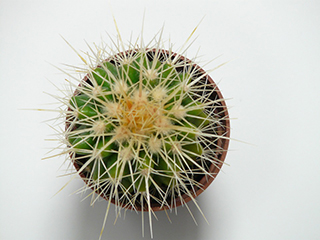
\includegraphics[width=1\linewidth]{figures/ball.jpg}
%   \caption{$\ell_p$ ball with $0 < p \ll 1$.}
%   \label{fig:flower}
% \end{marginfigure}
In the above general model, $\mathcal P(\w)$ is the penalty term, which simultaneously imposes both sparsity and structure (blobs). The different spatial regularization
methods that have appeared in neuro-imaging literature can be cast into this
correspond to different choices of the convex penalty $\mathcal P$ acting on the extended gradient of the coefficients $\w$. Viz,

\begin{equation}
  \begin{split}
  \mathcal P(\w) = \begin{cases}
    \rho\|\w\|_1 + \frac{1}{2}(1-\rho)\|\nabla \w\|_{\text{Fro}}^2 = \sum_{j \in [\![p]\!]}\rho|w_j| + \frac{1}{2}(1-\rho)\|(\nabla \w)_j\|_2^2, &\mbox{ for GraphNet
      %~\citep{grosenick2013,hebiri2011}
    },\\
    \|\nabla_\rho \w\|_{1+2,1} = \rho\|\w\|_1 + \|\nabla \w\|_{2,1} = \sum_{j  \in [\![p]\!]}\rho|w_j| + (1-\rho)\|(\nabla \w)_j\|_2, &\mbox{ for isotropic TV-$\ell_1$
      %~\citep{baldassarre2012,gramfort2013}
    },\\
    \|\nabla_\rho \w\|_{1,1} = \rho\|\w\|_1 + (1-\rho)\|\nabla \w\|_{1,1} = \sum_{j  \in [\![p]\!]}\rho|w_j| + (1-\rho)\|(\nabla \w)_j\|_1, &\mbox{ for anisotropic TV-$\ell_1$
    },\\
    \|\nabla_\rho \w\|_{2,1} = \sum_{j  \in [\![p]\!]}\|(\nabla_\rho \w)_j\|_2, &\mbox{ for Sparse Variation
      %~\citep{eickenberg2015total}
    },\\
      \vdots
    \end{cases}
  \end{split}
  \label{eq:penalty}
\end{equation}
where
\begin{itemize}
  \item $\alpha > 0$ is a regularization parameter controls the total amount of regularization;
\item $\rho$ ($0 < \rho \le 1$) is a mixing constant between
  the {sparsity-inducing} $\ell_1$ part and the
  {cluster-promoting} part of the penalty term.
  The particular case {$\rho = 1$} corresponds to the usual Lasso. Vanilla TV  ~\citep{michel2011tv} corresponds to TV-$\ell_1$ with $\rho = 0$.
\item The matrix $\nabla_\rho$ is the extended discrete gradient operator defined in the table of notations.
\end{itemize}
\begin{shaded}
\paragraph{Bayesian interpretation of SpaceNet models.} The penalties $\mathcal P(\w)$ in \eqref{eq:opt_pb} admit a Bayesian interpretation as a prior on the distribution of the coefficients $\w$
\begin{equation}
  \label{eq:bayesian}
  p_{\alpha,\rho}(\w) \propto \exp(-\mathcal P(\w)).
\end{equation}
For example, the GraphNet~\citep{grosenick2013,hebiri2011}, the penalties $\mathcal P(\w)$ penalty corresponds to
\begin{equation}
p_{\alpha,\rho}(\w) \propto    \prod_{j=1}^p\exp(-\alpha\rho |w_j|)\prod_{j=1}^p\exp\left(-\alpha(1-\rho)\sum_{l \sim \text{neigh}(j)}w_j\Delta_{j,l}w_l\right).
\end{equation}
\end{shaded}

\begin{marginfigure}
  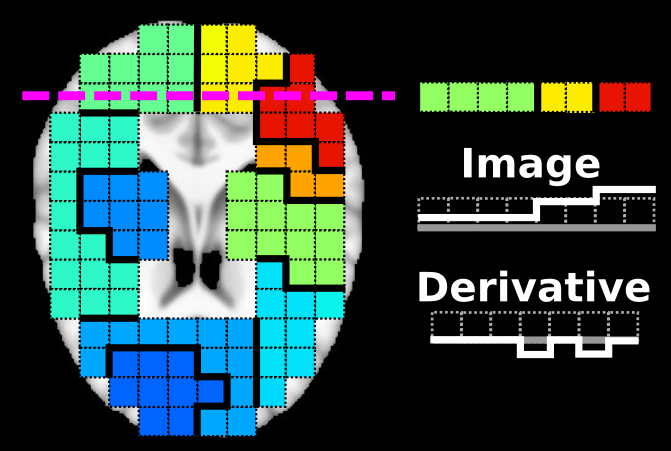
\includegraphics[width=1\linewidth]{figures/tv_cartoon_horizontal.png}
  \caption{A cartoon showing a sparse and blobby (step-wise constant / cartoon-like) brain map,
  as would be sought for by Total-Variation regularization \eqref{eq:ss}.}
  \label{fig:roi}
\end{marginfigure}

SpaceNet models \eqref{eq:main_pb} result brain maps which are both
sparse (i.e regression coefficients $\w$ are zero everywhere, except at
predictive voxels) and structured (blobby). See Fig. \ref{fig:roi}. The superiority of such
methods over methods without structured priors like the Lasso, ANOVA,
Ridge, SVM, etc. for yielding more intepretable maps and improved
prediction scores is now well established. See for example
 ~\citep{baldassarre2012,gramfort2013}. These priors are fast becoming
popular for brain decoding and segmentation. Indeed, they leverage a
feature-selection function
(since they limit the number of active voxels),
and also a structuring function
(since they penalize local
differences in the values of the brain map). For example, see Fig.
\ref{fig:spacenet_maps}.
Also, such priors produce state-of-the-art methods for automatic
extraction of functional brain atlases  ~\citep{abraham2013}.

\begin{shaded}
  \paragraph{Submodular interpretation of TV.} We note that anisotropic TV penalty \eqref{eq:penalty} on
  an arbitrary (undirected) graph $G = (V,E)$ is the \textit{Lovasz extension} of the \textit{cut-function}
  $F : 2^V \rightarrow \mathbb N$, $S \mapsto "\text{number of edges between } S \text{ and }V\setminus S"$,
defined by $F^L(x) := \mathbb E_{\lambda \sim \mathcal U([0,1])}[F(\{v \in V|x_v \ge \lambda\})]$, for all $x \in [0,1]^{\#V}$. Thus anisotropic TV can be seen as a graph-cut problem for which efficient algorithms exist~\citep{bach13sub,landrieu16}.
\end{shaded}

\section{Methods}
The SpaceNet model leads to difficult non-smooth mathematical optimization problems making their implementation and practical usability challenging.~\citep{dohmatob2014benchmarking} benchmarked a rich variety of cutting-edge solvers for such problems, and gave crucial recommendations on how to effectively implement these algorithms in practice. In these benchmarks, the FISTA algorithm emerged as the go-to algorithm for the TV-L1 problem~\citep{dohmatob2015speeding}. These hints have been carefully used in implementing SpaceNet. Also as a preprocessing step, we use univariate feature-screening (ANOVA) to eliminate voxels which are irrelevant to the learning problem, thus reducing the size of the problem. As a result the implementation of SpaceNet is fast, robust, and automatically sets its parameters (internal cross-validation). All these technical details will be properly presented in the next few chapters.

\subsection{Cross-validation}
Cross-validation (e.g see ~\citep{stone74}) is a technique used to protect against overfitting in a predictive model, particularly in a case where the amount of data may be limited. In cross-validation, you make a fixed number of folds (or partitions) of the data, run the analysis on each fold, and then average the overall error estimate. This gives an (asymptotically) unbiased estimate of the true generalization error of the model. 
Two major types of cross-validation are K-Fold and Leave-One-Out (LOO).

\paragraph{K-Fold cross-validation.}
One iteration of the K-fold cross-validation is performed in the following way: First, a random permutation of the sample set is generated and partitioned into K subsets ("folds") of about equal size. Of the K subsets, a single subset is retained as the validation data for testing the model (this subset is called the "testset"), and the remaining K - 1 subsets together are used as training data ("trainset"). Then a model is trained on the trainset and its accuracy is evaluated on the testset. Model training and evaluation is repeated K times, with each of the K subsets used exactly once as the testset.
The case of a 5-fold cross-validation with 30 samples is illustrated in Fig. \ref{fig:cv}.

\paragraph{Leave-One-Out cross-validation.}
As the name suggests, leave-one-out cross-validation involves using a single sample from the original sample set as the validation data, and the remaining samples as the training data. This is repeated such that each sample in the sample set is used exactly once as the validation data. This is the same as K-fold cross-validation where K is equal to the number of samples in the sample set.
In LOO, there is no need in generating random permutations and in repeating it, because the training and validation datasets for each of the folds are always the same, and therefore the result of the accuracy estimation is determined.

\begin{figure}
  \subfloat[1 iteration of 5-Fold cross-validation]{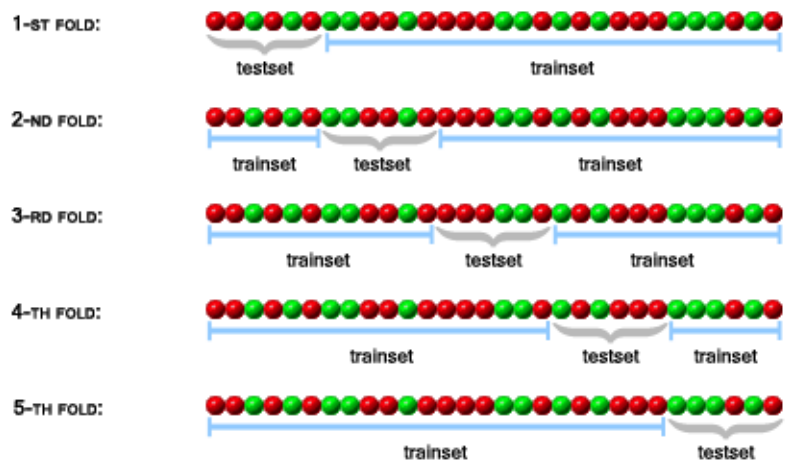
\includegraphics[width=1\linewidth]{figures/cv_folds.png}}\\
  \subfloat[Parameter grid]{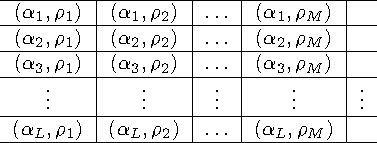
\includegraphics[width=1\linewidth]{figures/cv_grid.pdf}}
  \caption{\textbf{Model-selection} via cross-validation.
\textbf{\textit{(a)}} K-Fold cross-validation, illustrated
here for the case $K = 5$, involves
taking the available data and partitioning it into $K$ groups. Then
$K - 1$ groups are used to train a set of models that are then
evaluated on the remaining group. Adapted from \url{http://genome.tugraz.at/proclassify/help/pages/XV.html}.
\textbf{\textit{(b)}} $L \times M$ grid over which to search for optimal configuration in
a model with two hyper-parameters $\alpha$ and $\rho$. For a model like SpaceNet \eqref{eq:main_pb}, the grid is is constrained to verify $0 \le\alpha_L < \ldots < \alpha_1 = \alpha_{\text{max}}$ and $0 \le \rho_M < \ldots < \rho_1 \le 1$, with $L = 10$ and $M = 3$ typically, given a total of $LM = 30$ models to compare. In chapter \ref{chap:speeding}, we show how \textit{early-stopping} and other heuristics can be used to make the total cost much more effective than just fitting $LM$ models in a CV loop. }
  \label{fig:cv}
\end{figure}

\paragraph{Model-selection via cross-validation.}
One can instrument cross-validation to tune the hyper-parameters of a model like SpaceNet \eqref{eq:main_pb}, by selected the configuration of model parameters with least cross-validation error. The number of models fitted is proportional to the size of the parameter grid --i.e exponential in the number of parameters to tune-- and therefor can become prohibitive in case there are many free hyper-parameters in the model. Also, since some of the data has to be set aside for validation, cross-validation in very small sample settings (e.g e few tenths, as is the in some neuroimaging experiments) may be troublesome as the error estimates then have very high variance. A reasonable alternative in such situations are SURE (short for \textit{Stein's Unbiased Risk Estimator}~\citep{stein1981})-based methods,
which are applicable whenever a procedure for obtaining (an unbiased estimate of) the number of degrees of freedom of the model is available. This is the case with the models like the ElasticNet and
GraphNet~\citep{hebiri2011}. Recently, ~\citep{sugar} has proposed a STEIN-based technique for structured models with many hyper-parameters.


\subsection{How SpaceNet compares against classical unstructured models}
\paragraph{Classification.}
We compared SpaceNet (TV-L1 and GraphNet / Smooth-Lasso priors) with an SVM (Support Vector Machine) on the visual-recognition dataset~\citep{haxby2001}. This dataset consists of 6 subjects with 12 runs per subject. In each run, the subjects passively viewed images of eight object categories, grouped in 24-second blocks separated by intermittent rest periods. This experiment is a classification task: predicting the object category. The design matrix is made of time-series from the full-brain mask of $p=23,707$ voxels over 216 TRs (Repetition Times), of a single subject (subj1). 126 TRs were used for training all the models, whilst testing was done on 90 left-out TRs. The results are depicted in Figures \ref{fig:spacenet_maps} and \ref{fig:spacenet_bars}.

\paragraph{Regression.}
In ~\citep{gramfort2013}, the authors compared several models on a dataset in which subjects were presented with mixed (gain/loss) gambles, and decided whether they would accept each gamble~\citep{jimura2012}. No outcomes of these gambles were presented during scanning, but after the scan three gambles were selected at random and played for real money. The prediction task here is to predict the magnitude of the gain and thus a regression on a continuous variable. The full dataset of 16
subjects with 48 3D scans each, making up for a total of $n=768$ samples with approximately $p=3.3 \times 10^4$ voxels. The prediction here is inter-subject: the estimator
learns on some subjects and predicts on left out subjects.
The results are shown in Fig. \ref{fig:tvl1_regression}.

\begin{pagefigure}%[!htb] 
  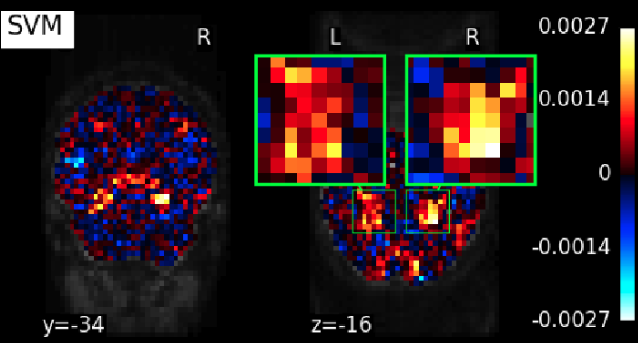
\includegraphics[width=.32\linewidth]{figures/svm.png}
  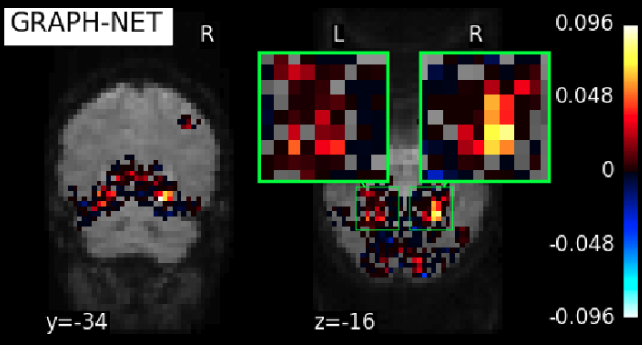
\includegraphics[width=.32\linewidth]{figures/graphnet.png}
  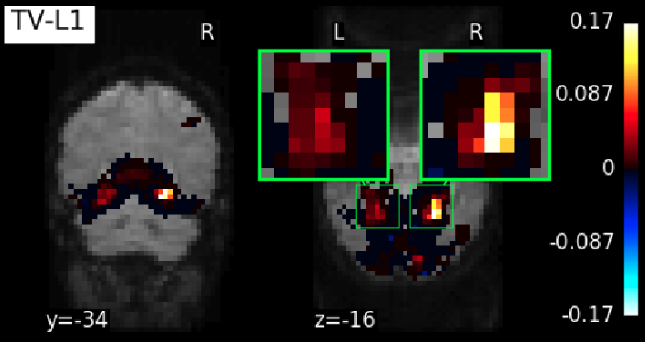
\includegraphics[width=.32\linewidth]{figures/tvl1.png}  
  \caption{The figure shows results of comparing the SpaceNet  models TV-$\ell_1$ and
    Graph-Net against an SVM (Support Vector Machine) classifier on
    the visual-recognition dataset  ~\citep{haxby2001}
    As can be seen from the figure, SpaceNet priors (TV-$\ell_1$, GraphNet, etc.)
    yield stable and more intepretable maps by enforcing smoothness on the coefficients while segmenting predictive regions (blobs) from noisy background.}
  \label{fig:spacenet_maps}
\end{pagefigure}
\begin{figure}[!htbp]
  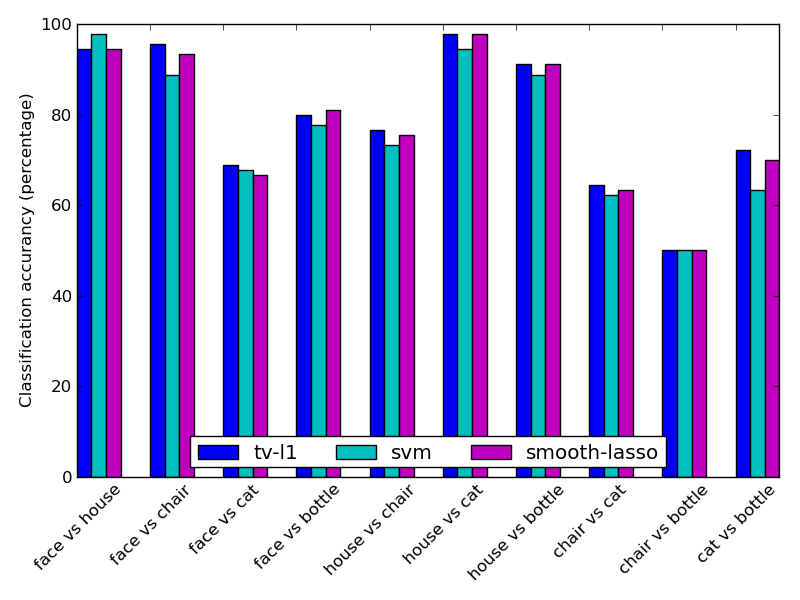
\includegraphics[width=1\linewidth]{figures/haxby_barchart.png}
  \caption{Bar chart showing percentage classification on leftout, for one-vrs-one classification on the visual recognition dataset~\citep{haxby2001}.
  }
  \label{fig:spacenet_bars}
\end{figure}

\section{Conclusion}
We have presented SpaceNet, a family of priors for brain decoding that enforce both sparsity and structure, leading to better prediction scores and intepretable brain maps. We believe that such priors will become commonplace in future.
In the next few chapters, we open the ``black-box'' and develop from ground-up, the details of such models, including their practical implementation on a computer.

\begin{figure}[!htbp] 
  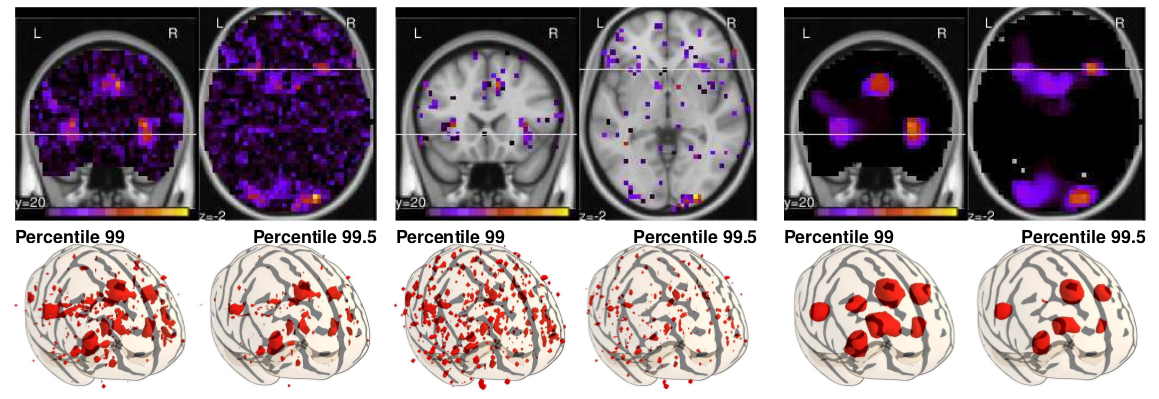
\includegraphics[width=1\linewidth]{figures/gramfort_tvl1.png}
  \caption{Results on fMRI data from [4] (from left to right F-test, ElasticNet and TV-L1). The TV-L1 regularized model segments neuroscientifically
    meaningful predictive regions in agreement with univariate statistics while the ElasticNet yields sparse although very scattered non-zero weights. Source: adapted from ~\citep{gramfort2013}.}
  \label{fig:tvl1_regression}
\end{figure}

% \clearpage
\bibliographystyle{plainnat}
\bibliography{bib_all}
